\chapter{Entity Relational Diagrams}

Entity Relational Diagrams are a visual diagramming language for
describing entities using relational vocabulary.

To describe an entity, we draw a rectangle in which we write
emphasized on the first line the name of the entity, and on the
remaining lines the attributes of the entity.  

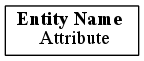
\includegraphics{figs/entity.png}

If it is a strong entity, we underline its natural key.  

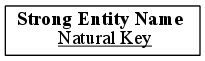
\includegraphics{figs/strong_entity.png}

If it is a weak entity, we dashed underline its discriminator (or weak
key), and draw a second rectangle around the first.

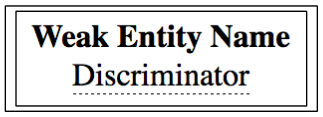
\includegraphics[scale=0.7]{figs/weak_entity.png}

A variation is to write the attributes in ovals connected to the
entity by lines.

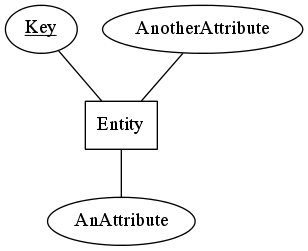
\includegraphics[scale=0.8]{figs/alternate_entity.png}

\newpage

To describe a relationship between two entities, we draw a rhombus in
which we write the name of the relationship.  We then draw lines
between the rhombus and the entities it relates.  We double the line
between an entity and the relationship if the entity can't exist
without being part of such a relationship.  We further decorate the
lines with cardinality: ``1'' meaning exactly one of this entity
relates to one or many of the other entity in the relationship, ``n''
meaning many of this entity relates to one or many of the other entity.

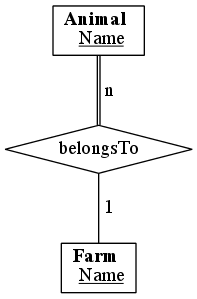
\includegraphics{figs/relationship.png}

We can also specify minima and maxima by ``(min,max)''.  If the
relationship itself has attributes, they will be drawn in ovals
connected to the relationship by a line.
